\documentclass{article}
\usepackage{pdfpages}
\usepackage{graphicx}  % For PNG
\usepackage[left=2cm, right=2cm, top=2cm]{geometry}
\usepackage{minted}
% Give Table of Contents Hyperlinks
\usepackage{hyperref}
\hypersetup{
    colorlinks,
    citecolor=black,
    filecolor=black,
    linkcolor=black,
    urlcolor=blue
}
\pagenumbering{gobble}
% \pagenumbering{roman} % set the numbering style to lowercase letter

\title{\textbf{Homework 5}}

\author{MacMillan, Kyle}
\date{November 26, 2018}

\begin{document}


\addcontentsline{toc}{section}{Title}
\maketitle

\newpage
\tableofcontents
\addcontentsline{toc}{section}{Table of Contents}
\newpage
\listoffigures
\addcontentsline{toc}{section}{List of Figures}

\pagenumbering{roman}   % Set TOC page numbering to lowercase roman numerals


%%%%%%%%%%%%%%%%%%%%%%%%%%%% INTRO SECTION %%%%%%%%%%%%%%%%%%%%%%%%%%%%
\newpage
\hypersetup{
    colorlinks,
    citecolor=blue,
    filecolor=black,
    linkcolor=blue,
    urlcolor=blue
}
\pagenumbering{arabic}  % Set content page numbering to arabic numerals

\setcounter{page}{1}
\newpage
\section{\textbf{Chapter 11}}
\subsection{Problem 3}
Write a Python program to navigate a robot using the Wavefront algorithm. Demonstrate on a map with multiple obstacles.


% \begin{figure}[h]
%     \centering
%     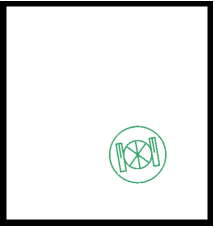
\includegraphics[pages=1]{stuck1}
%     \caption{Problem 5.2 Stuck Robot}
%     \label{fig:stuck1}
% \end{figure}

\newpage
\section{\textbf{Chapter 16}}
\subsection{Problem 1}
asdf

\subsection{Problem 2}
asdf

\newpage
\section{\textbf{Chapter 17}}
\subsection{Problem 2}
asdf


\subsection{Problem 3}
asdf


\subsection{Problem 4}
asdf



\newpage
\section{\textbf{Chapter 18}}
\subsection{Problem 1}
\subsubsection{Problem 1.1}
asdf


\subsubsection{Problem 1.2}
asdf


\subsubsection{Problem 1.3}
asdf


\end{document}
